\documentclass[amsmath, amssymb, aps, floatfix, nofootinbib, preprintnumbers,
  showpacs, superscriptaddress, twocolumn]{revtex4-1}
\usepackage{bm}
\usepackage{graphicx}
\usepackage{hyperref}
\usepackage[cmyk]{xcolor}
\bibliographystyle{apsrev4-1}
\begin{document}

\title{The Berggren basis in elastic scattering}
\date{\today}

\author{Fei Yuan}
\email[E-mail: ]{yuan@nscl.msu.edu}
\affiliation{National Superconducting Cyclotron Laboratory and
             Department of Physics and Astronomy,
             Michigan State University,
             East Lansing, MI 48824, USA}

\begin{abstract}
  We describe the theory of the Berggren basis, which unites bound, resonant,
  and continuum states under a single consistent framework, and demonstrate
  its utility by calculating the resonance in the \textsuperscript{11}Be halo
  nucleus using a simple Woods--Saxon model.  The basis is generated by
  applying the contour deformation method and diagonalizing the discretized
  Schr\"odinger equation in momentum space.  We show that the energy obtained
  are comparable in accuracy to the differential equations approach, although
  the asymptotic behavior does not appear to be adequately described.
\end{abstract}
\maketitle

\newcommand{\D}{\operatorname{d \!}\mathord{}}
\newcommand{\E}{\mathrm e}
\newcommand{\I}{\mathrm{i}}
\newcommand{\PI}{\pi}

\section{Introduction}

Resonances play an important role in the understanding of many quantum
systems.  They are an intrinsic property of the systems and describe the
energies at which cross sections are strongly enhanced.\cite{Michel2009}

Formally, resonances appear as poles of the S-matrix in the complex momentum
plane.\cite{Newton1966} As states with complex momenta, they are not directly
observable.  However, if the width is sufficiently small, they can become
close enough to the real momentum axis that they imprint themselves on the
physical reactions, resulting in the characteristic arctangent phase shift.

Resonant states, sometimes referred to as Gamow states, are not part of the
standard quantum mechanical framework due to their non-normalizability through
the L\textsuperscript{2}-norm.  However, with the development of the rigged
Hilbert space and its associated nonhermitian formalism of quantum mechanics,
the concept of resonances has been made fully rigorous.\cite{Bohm1978}.

Unified with bound and continuum states under one framework through the
Berggren completeness relation,\cite{Berggren1968} resonance states form a
useful building block for many-body theories such as the Gamow shell
model\cite{Hagen2006}, the Gamow-Hartbree-Fock-Bogoliubov
method,\cite{Michel2008} and the complex coupled-cluster
method.\cite{Hagen2007} All of these methods make use of the unique properties
of resonant states to enable calculations of nuclei far from stability.

In this paper, we demonstrate the utility of the Berggren formalism in the
calculation of a simple elastic scattering problem through the basis expansion
method.  We make use of the contour deformation method to construct the
Berggren basis, as described in \cite{Hagen2005} and \cite{Bengtsson2013}, in
which the Schr\"odinger equation is analytically continued into the complex
plane.

The numerical calculations are performed using a combination of Python and C
code, making use of the Numpy, Scipy, and Slatec libraries.  The code for this
project has been made public available on
GitHub.\footnote{\url{https://github.com/xrf/phy982-proj}}

\section{Theory}

\subsection{General setup}

We shall consider a simple scattering problem in which two particles interact
via a spherically symmetric potential $V$, defined as a function of the
relative coordinate $\bm R$.  The interaction is assumed to be short-ranged
and should thus become negligible after a finite radius (this excludes Coulomb
interactions).  The Schr\"odinger equation for such a system is given
by:\footnote{For clarity, we use natural units where $\hbar = 1$.}
\begin{align} \label{eq:0}
  -\frac{1}{2 \mu} \nabla_{\bm R}^2 \psi(\bm R) + V(R) \psi(\bm R) = E \psi(\bm R)
\end{align}
where $\mu$ is the reduced mass of the system and $E = k^2 / (2 \mu)$ is the
energy of the eigenstate.

The standard approach to solving such a problem is to use separation of
variables to decompose the wave function into a sum of partial waves, each
identified by orbital angular momentum $\ell$ and its $z$-projection $m$.
Since this is a scattering problem, we may also assume azimuthal symmetry by
aligning the the incident beam with the $z$-axis, allowing us to ignore all
but the $m = 0$ partial waves:
\begin{align*}
  \psi(\bm R) = \sum_{\ell = 0}^\infty c_{\ell} \frac{u_\ell(R)}{R} Y_\ell^0(\hat{\bm R})
\end{align*}
where $c_{\ell}$ are coefficients, $u_\ell$ is some radial wave function,
and $Y_\ell^m$ are spherical harmonics.

\subsection{Radial solutions}

The radial wave function $u_\ell$ may be obtained by solving the
Schr\"odinger-like equation:\cite{Thompson2009}
\begin{align} \label{eq:1}
  -\frac{1}{2 \mu} \frac{\D^2}{\D R^2} u_\ell(R)
  + V_\ell^{\text{eff}}(R) u_\ell(R)
  = E u_\ell(R)
\end{align}
where the effective potential $V_\ell^{\text{eff}}$ adds an additional
centrifugal term:
\begin{align*}
  V_\ell^{\text{eff}}(R) = V(R) + \frac{\ell (\ell + 1)}{2 \mu R^2}
\end{align*}
Equation \eqref{eq:1} admits four different categories of solutions, known as
bound, scattering, resonant, and antibound states, the choice of which depends
on the boundary conditions imposed on the equation.

In bound states, the radial part $u(R)$ rapidly approaches $0$ as
$R \to \infty$ and are thus L\textsuperscript{2}-normalizable.  Specifically, its
asymptotics behave like:
\begin{align*}
  u(R) \sim \E^{-\kappa R}
\end{align*}
From the perspective of scattering, these may be formally treated as outgoing
waves with imaginary momentum $k = \kappa \I$.  They form a discrete spectrum
of energies, all of which are negative.

In scattering states, the radial part $u(R)$ do not approach $0$ and thus
cannot be normalized in the usual sense.  Their asymptotics behave as
spherical waves:
\begin{align*}
  u(R) \sim \E^{\pm \I k R}
\end{align*}
They can be either incoming ($-$) or outgoing ($+$) and are characterized by
positive momenta $k$.  The states form a continuous spectrum and thus are
often referred to as ``continuum states'', although we shall reserve the
latter term for the more general set of states with complex momenta.

Resonance states have characteristics of both scattering and bound states:
they form a discrete spectrum yet they are not normalizable as their
asymptotics grow exponentially:
\begin{align*}
  u(R) \sim \E^{(\pm k - \I \kappa) \I R}
\end{align*}
The sign determines whether they are capture ($-$) or decay ($+$) resonances,
which are analogous to incoming and outgoing waves respectively, and they
affect the temporal behavior of the wave function: the former grows over time
while the latter decays over time.  In particular, they always occur in pairs:
for every decay resonance $k - \I \kappa$ there is a corresponding capture
resonance $-k - \I \kappa$.  The complex energy of such a resonance state
describes two essential properties of the resonance:
\begin{align*}
  E_{\text r} - \frac{\Gamma}{2} \I = \frac{(k - \I \kappa)^2}{2 \mu}
\end{align*}
Here, $E_{\text r}$ is the resonance energy and $\Gamma$ is the width, which
quantifies the lifetime of this state.  Physically relevant states -- those
that have a noticeable effect on cross sections -- generally satisfy
$\Gamma \ll E_{\text r}$.

Antibound states are in a way dual to bound states.  They too appear as a
discrete spectrum and have imaginary momenta, but the momenta have the
opposite sign and thus the wave functions grow exponentially:
\begin{align*}
  u(R) \sim \E^{\kappa R}
\end{align*}
Antibound states are difficult to interpret\cite{Michel2009}, although they do
subtly manifest themselves in certain physical phenomena.  Although we do not
make use of them in this paper, the Berggren formalism can be generalized to
include antibound states as well.\cite{Vertse1989}

\begin{figure}
  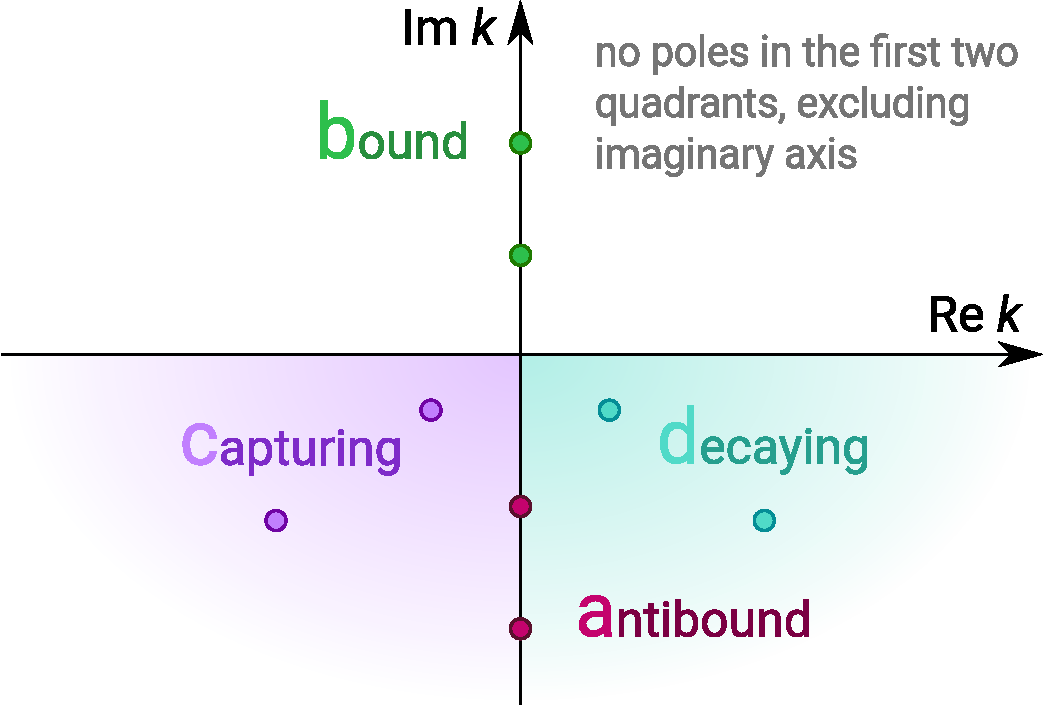
\includegraphics[width=.4\textwidth]{proj-poles.pdf}
  \caption{Poles in the S-matrix on the complex momentum plane.}
  \label{fig:1}
\end{figure}

These four kinds of states can be represented graphically as points on the
complex momentum plane, as depicted in Figure \ref{fig:1}.  The bound,
resonant, and antibound states appear as poles in the S-matrix, while all the
points on the real axis denote scattering states.

\subsection{Berggren basis}

A well-known theorem of scattering theory states:
\begin{align*}
\sum_{k \in \text{bound}} |u_k\rangle \langle u_k|
+ \int_0^\infty |u(k)\rangle \langle u(k)| \D k = \hat 1
\end{align*}
where $u_k$ are non-scattering wave functions (such as bound states) and
$u(k)$ are the momentum space scattering wave functions.  This is known as the
Newton completeness relation\cite{Newton1966} and allows bound and scattering
states to be unified into one basis in which all solutions of \eqref{eq:1} can
be expanded.

\begin{figure}
  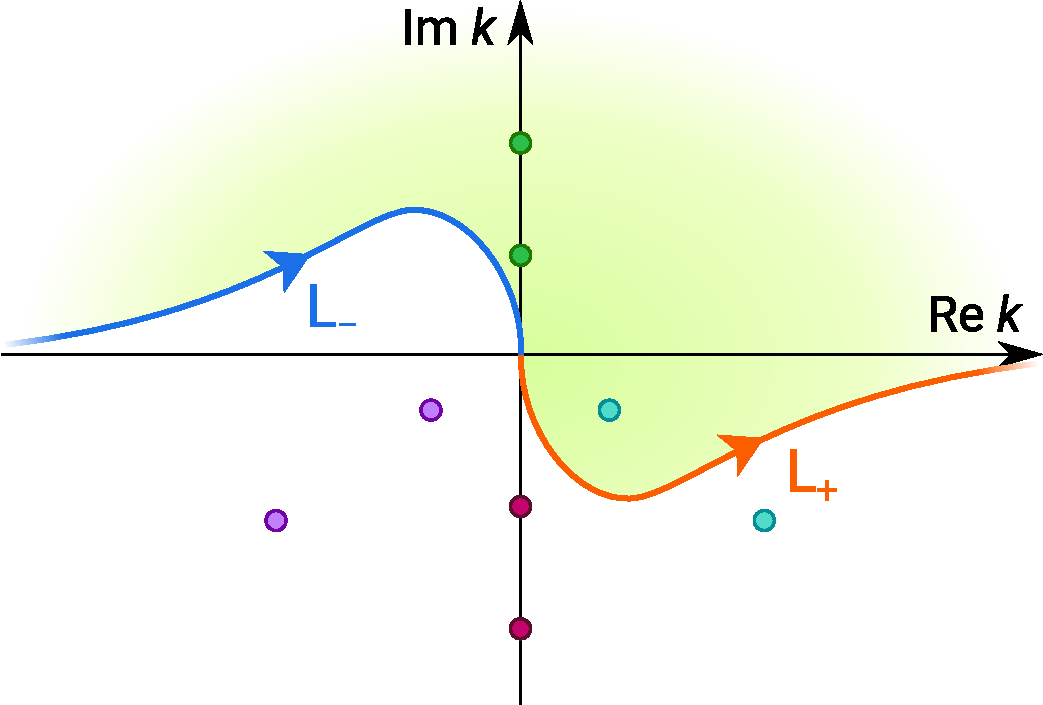
\includegraphics[width=.4\textwidth]{proj-completeness.pdf}
  \caption{A contour that may be used in the Berggren completeness relation.}
  \label{fig:2}
\end{figure}

However, the relation does not include resonance states.  This can be remedied
by choosing an alternative path for the integral, such as $L_+$ contour shown
in \ref{fig:2}.  This leads to the Berggren completeness relation:\cite{Berggren1968}
\begin{align} \label{eq:2}
\sum_{\substack{k \in \text{bound},\\\text{resonant}}} |u_k\rangle \langle u_k|
+ \int_{\mathrm L_+} |u(k)\rangle \langle u(k)| k^2 \D k = \hat 1
\end{align}
where the sum over discrete states contains both bound and resonant states
that lie above the $\mathrm L_+$ contour.  The integral over scattering states
has been changed to an integral over continuum states, which have complex
momenta.  Such a basis, which includes resonant states in addition to bound
and continuum states, is referred to as a Berggren basis.

The exponentially divergent nature of states in a Berggren basis pose a
serious problem for the computation of norms and matrix elements, both of
which involve integrating the states from $R = 0$ to $R = \infty$.
Fortunately, there are ways to overcome the divergence using regularization
techniques.

Zel'dovich proposed\cite{Zeldovich1960} a technique in which the integrand is
multiplied by a Gaussian function $\E^{-\varepsilon R^2}$, which suppresses
the divergence at large $R$.  Afterwards, the $\varepsilon \to 0$ limit may be
taken, hoping that a finite result is returned.  The same technique was used
by Berggren to prove the completeness theorem \eqref{eq:2}.

Alternatively, one may use exterior complex scaling, in which the outer part
of the radial integration contour is deformed so that it approaches infinity
at an angle for which the integral converges.\cite{Gyarmati1971}

\subsection{Momentum-space Schr\"odinger equation}

To solve for resonant states, it is convenient to use the momentum-space
version of the Schr\"odinger equation.  First, we define the eigenfunctions
$\phi_{\bm k}$ of momentum $\bm k$, which are simply plane waves:
\begin{align*}
  \phi_{\bm k}(\bm R) = \frac{1}{(2 \PI)^{3/2}} \E^{\I \bm k \cdot \bm R}
\end{align*}
The coefficient of the functions has been chosen to satisfy
\begin{align*}
  \int_{\mathbb R^3} \phi_{\bm k^*}^*(\bm R) \phi_{\bm k'}(\bm R) \D^3\!\bm R
  = \delta(\bm k - \bm k')
\end{align*}
where $\delta$ is the Dirac delta distribution.  One may consider this to be a
form of normalization, although this is not the standard
L\textsuperscript{2}-norm.

A wave function in position space $\psi$ may be converted into its
corresponding wave function in momentum space $\tilde \psi$ via the Fourier
transform:
\begin{align} \label{eq:3}
  \tilde \psi(\bm k) =
  \int_{\mathbb R^3} \phi^*_{\bm k^*}(\bm R) \psi(\bm R) \D^3\!\bm R
\end{align}
Given the symmetries of the problem, it would be useful to factor out the
angular components of the transformation.  To do this, we apply the plane wave
expansion to $\phi_{\bm k}$:\cite{Mehrem2011}
\begin{align*}
  \phi_{\bm k}(\bm R) = \sum_{\ell = 0}^\infty \sum_{m = -\ell}^\ell
  \frac{s_\ell(k R)}{k R} Y_\ell^m{}^*(\hat{\bm k}) Y_\ell^m(\hat{\bm R})
\end{align*}
where $s_\ell$ is a rescaled Riccati--Bessel function defined by
\begin{align*}
  s_\ell(z) = \sqrt{\frac{2}{\PI}} \I^\ell z j_\ell(z)
\end{align*}
and $j_\ell$ is the spherical Bessel function of order $\ell$.  Physically,
$s_\ell(k R)$ are partial wave scattering states of \eqref{eq:1} when the
interaction $V$ is absent.  Substituting the expansion into \eqref{eq:3} and
assuming azimuthal symmetry gives:\footnote{In the original presentation, we
  used a different definition of the momentum wave function $\varphi_\ell$,
  which is related to the current definition via
  $\varphi_\ell(k) = \tilde u_\ell(k) / k$.}
\begin{align*}
  \tilde \psi(\bm k) =
  \sum_{\ell = 0}^\infty c_\ell \frac{\tilde u_\ell(k)}{k} Y_\ell^0(\hat{\bm k})
\end{align*}
where
\begin{align*}
  \tilde u_\ell(k) = \int_0^\infty s^*_\ell(k^* R) u_\ell(R) \D R
\end{align*}
is the momentum-space analog of $u_\ell$.  The position-space wave function
can also be recovered from $\tilde u_\ell(k)$ by performing the inverse
transform:
\begin{align*}
  u_\ell(k) = \int_0^\infty s_\ell(k R) \tilde u_\ell(k) \D k
\end{align*}

Similarly, an interaction in position space $U$ can be transformed into its
momentum-space version $\tilde U$ via a Fourier-like transform:
\begin{align*}
  \tilde U(\bm k, \bm k') = \int_{\mathbb R^3}
  \phi^*_{\bm k^*}(\bm R) U(\bm R) \phi_{\bm k}(\bm R) \D^3\!\bm R
\end{align*}
For a spherically symmetric interaction, that is, $U(\bm R) = V(R)$, the plane
wave expansion can be used to factor out the angular components in the same
manner:
\begin{align*}
  \tilde U(\bm k, \bm k') = \sum_{\ell = 0}^\infty \sum_{m = -\ell}^\ell
  Y_\ell^m(\hat{\bm k}) \frac{\tilde V_\ell(k, k')}{k k'} Y_\ell^m{}^*(\hat{\bm k}')
\end{align*}
where
\begin{align} \label{eq:intv}
  \tilde V_\ell(k, k') = \int_0^\infty s^*_\ell(k^* R) V(r) s_\ell(k' R) \D R
\end{align}
In practical calculations, the integral \eqref{eq:intv} is usually performed
up to a certain cut-off $R_{\text{max}}$.

To obtain the momentum-space equation, we apply the Fourier transform in
\eqref{eq:3} to equation \eqref{eq:0}:
\begin{align*}
  \frac{1}{2 \mu} k^2 \tilde \psi(\bm k)
  + \int_{\mathbb R^3} \tilde U(\bm k, \bm k') \tilde \psi(\bm k') \D^3 k'
  = E \tilde \psi(\bm k)
\end{align*}
We then make use of the previous results to derive the Schr\"odinger equation
in momentum space for each partial wave in a spherically symmetric potential:
\begin{align} \label{eq:msse}
  \frac{1}{2 \mu} k^2 \tilde u_\ell(k)
  + \int_0^\infty \tilde V_\ell(k, k') \tilde u_\ell(k') \D k'
  = E \tilde u_\ell(k)
\end{align}

\section{Implementation}

\subsection{The \textsuperscript{11}B\lowercase{e} system}

We shall consider the \textsuperscript{11}Be halo nucleus, which may be
modeled by a valence neutron on top of an inert \textsuperscript{10}Be core
(mass number $A = 10$).  The interaction between the bodies is described by a
simple Woods--Saxon potential
\begin{align*}
  V(R) = \frac{V_0}{1 + \E^{(R - R_{\text{ws}}) / a_{\text{ws}}}}
\end{align*}
where the radius $R_{\text{ws}} = 1.2 A^{1/3}\,\mathrm{fm}$, the diffuseness
$a_{\text{ws}} = 0.65\,\mathrm{fm}$, and depth $V_0 = -61.1\,\mathrm{MeV}$.
The reduced mass of this system is
$\mu = \frac{1}{2} \times 0.0478450\,\mathrm{MeV}^{-1}\,\mathrm{fm}^{-2}$.

\subsection{Contour deformation}

\begin{figure}
  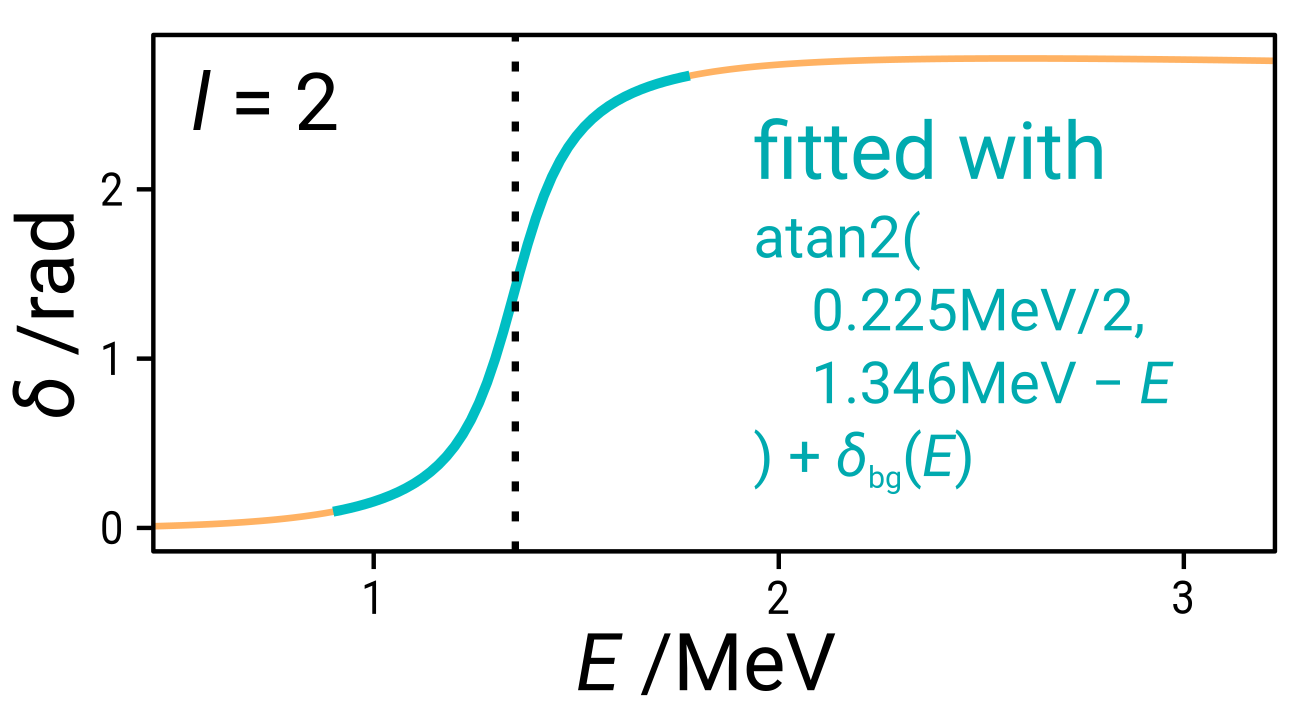
\includegraphics[width=.4\textwidth]{proj-atan.pdf}
  \caption{Fitting the energy dependence of the phase shift with
    $\operatorname{atan2}(\Gamma/2, E_{\text r} - E)$ to obtain the resonance
    parameters.}
  \label{fig:atan}
\end{figure}

To obtain a Berggren basis with complex momenta, the integration contour of
\eqref{eq:msse} must deformed to some new contour $\mathrm L_+$ so as to
enclose at least one resonant state:
\begin{align} \label{eq:dmsse}
  \frac{1}{2 \mu} k^2 \tilde u_\ell(k)
  + \int_{\mathrm L_+} \tilde V_\ell(k, k') \tilde u_\ell(k') \D k'
  = E \tilde u_\ell(k)
\end{align}
This requires some \textit{a priori} knowledge of where the state is likely to
be found.

Fortunately, we have previously solved the \textsuperscript{11}Be system using
the standard approach of applying a differential equation solver and matching
the asymptotic boundary conditions to obtain the partial wave S-matrix
elements and phase shifts.  From this calculation, a resonance of energy
$E_{\text r} = 1.346\,\mathrm{MeV}$ and width $\Gamma = 0.225\,\mathrm{MeV}$
was found for the $\ell = 2$ partial wave, as shown in Figure \ref{fig:atan}.
We thus expect to find a resonant state with the same parameters.

The contour we choose shall be a simple piecewise-linear contour from $k_0$ to
$k_{\text a}$ to $k_{\text b}$ to $k_{\text{max}}$.  The initial $k_0$ is a
positive value close to zero, but not exactly zero to avoid divergences in the
evaluation of the spherical Bessel function.  The point $k_{\text a}$ is
chosen to lie somewhere in the fourth quadrant, deforming the contour so as to
enclose the resonant state.  The point $k_{\text b}$ lies on the real axis,
bringing the contour back.  Finally, the point $k_{\text{max}}$, still on the
real axis, ends the contour and is thus the maximum momentum contained within
the basis.  Ideally, $k_{\text{max}}$ should be as large as is necessary to
obtain an acceptable result.

\subsection{Discretization of the contour}

To perform the calculation numerically, the integral in \eqref{eq:dmsse} must
be converted into a discrete sum.  There are many ways in which this can be
done.  We shall use the quadrature technique, which allows analytic integrals
to be approximated well with a finite, carefully chosen set of points
(``nodes'') $\kappa$ and weights $w_\kappa$:
\begin{align*}
  \int_{L_+} \tilde V_\ell(k, k') \tilde u_\ell(k') \D k'
  \approx \sum_{\kappa \in \mathrm L_+}
  \tilde V_\ell(k, \kappa) \tilde u_\ell(\kappa) w_\kappa
\end{align*}
Since contour is defined in terms of three linear pieces, we shall apply the
quadrature rule to each of the three segments separately.  The quadrature
scheme that we use is the standard Gauss--Legendre quadrature scheme, good for
smooth polynomial-like functions.

After discretization, the equation \eqref{eq:dmsse} takes on the following
form:
\begin{align*}
  \frac{1}{2 \mu} k^2 \tilde u^\ell_k
  + \sum_{\kappa \in \mathrm L_+}
  \tilde V^\ell_{k\kappa} \tilde u^\ell_\kappa w_\kappa
  = E \tilde u^\ell_k
\end{align*}
which can be solved as an eigenvalue problem
\begin{align*}
  \sum_{\kappa \in \mathrm L_+} \tilde H^\ell_{k \kappa} \tilde u^\ell_\kappa
  = E \tilde u^\ell_k
\end{align*}
with a Hamiltonian matrix
\begin{align*}
  \tilde H^\ell_{k \kappa} =
  \frac{1}{2 \mu} k^2 \delta_{k\kappa} + \tilde V^\ell_{k\kappa} w_\kappa
\end{align*}
Note that the Hamiltonian matrix is not hermitian, which prevents the use of
the efficient hermitian algorithms.  Despite this, the matrix can still be
rewritten into a complex-symmetric form, which may allow for some
optimizations.\cite{BarOn1998}

\section{Results}

\subsection{Resonant state}

\begin{figure}
  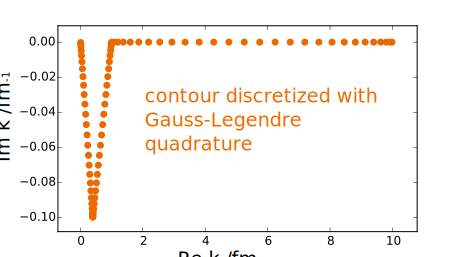
\includegraphics[width=.4\textwidth]{proj-contour.pdf}
  \caption{A discretized Gauss-Legendre contour with 80 points.}
  \label{fig:contour}
\end{figure}

Figure \ref{fig:contour} shows the typical discretized contour that is used in
our calculations.  The points are not evenly spaced; in particular, the points
are denser near the endpoints, which is typical for Gauss-Legendre quadrature.

The contour is chosen specifically to enclose the expected resonance at
$E_{\text r} = 1.346\,\mathrm{MeV}$ for the $\ell = 2$ partial wave, whose
complex momentum is approximately $(0.254 - 0.011\I)\mathrm{fm}^{-1}$.

\begin{figure}
  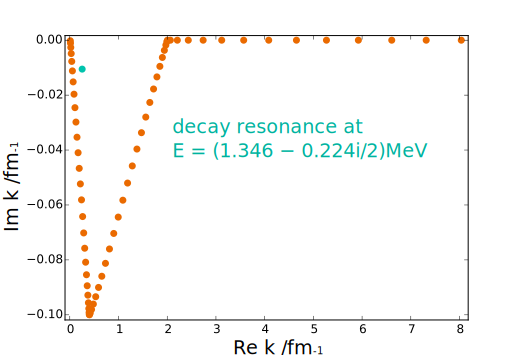
\includegraphics[width=.4\textwidth]{proj-l2.pdf}
  \caption{Momenta of the Berggren basis states for the $\ell = 2$ partial
    wave.}
  \label{fig:l2}
\end{figure}

\begin{figure}
  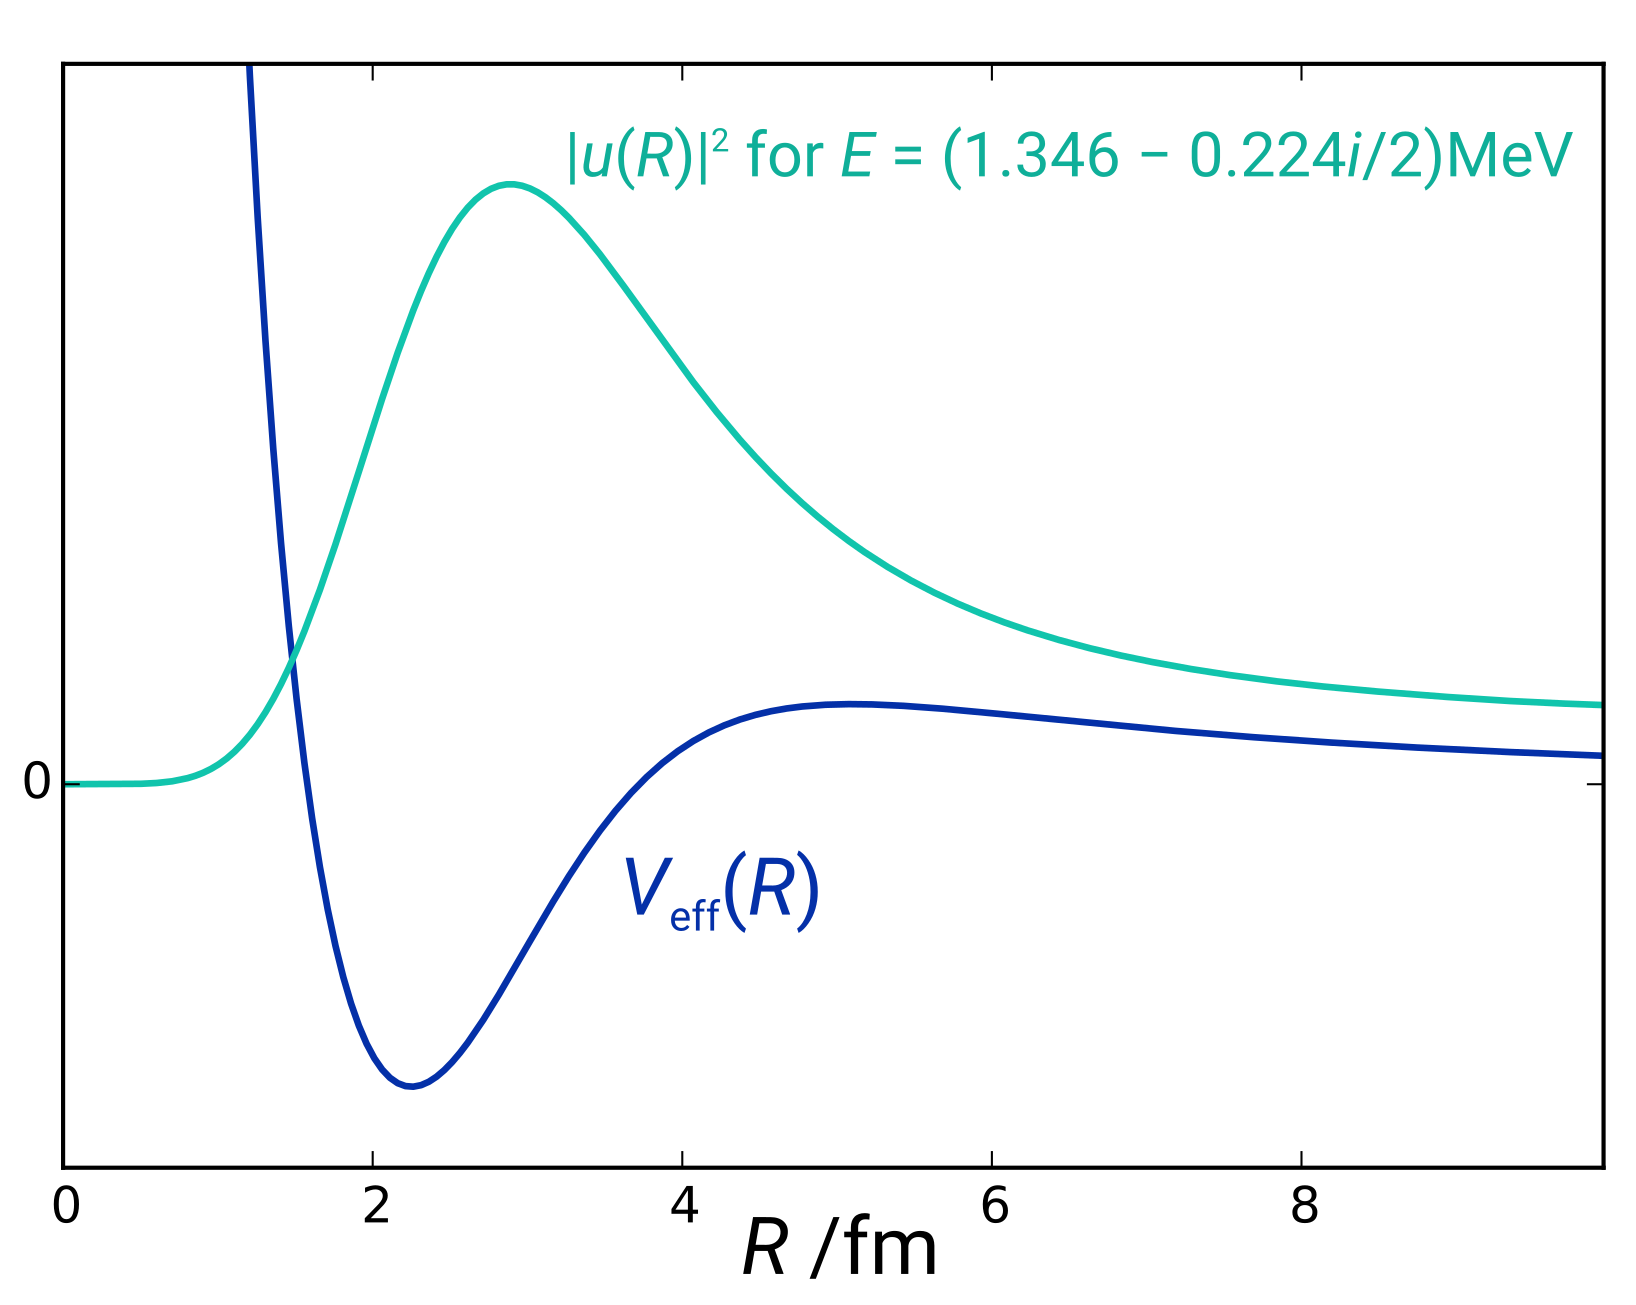
\includegraphics[width=.4\textwidth]{proj-l2-resonance.pdf}
  \caption{Resonant state for the $\ell = 2$ partial wave.}
  \label{fig:l2-resonance}
\end{figure}

After diagonalization, the energy eigenvalues are plotted in Figure
\ref{fig:l2}.  The majority of the points line on the original contour: these
are the continuum states in the Berggren basis.  However, there is one state
that lies outside the contour, indicating that it is likely a resonant state.
The position-space wave function of this resonant state, plotted in Figure
\ref{fig:l2-resonance}, is remarkably similar to a bound state like behavior
when $R$ is small.

The complex momentum of this resonant state is
$(0.254 - 0.011\I)\mathrm{fm}^{-1}$ and its complex energy is
$(1.346 - 0.224\I/2)\mathrm{MeV}$, both of which are in agreement with the
previous results, albeit with a slight discrepancy in the width of around
$0.001\,\mathrm{MeV}$.  This could be attributed to either uncertainties in
the previous result, perhaps due to a fitting error, or those in the current
result.

\subsection{Convergence}

\begin{figure}
  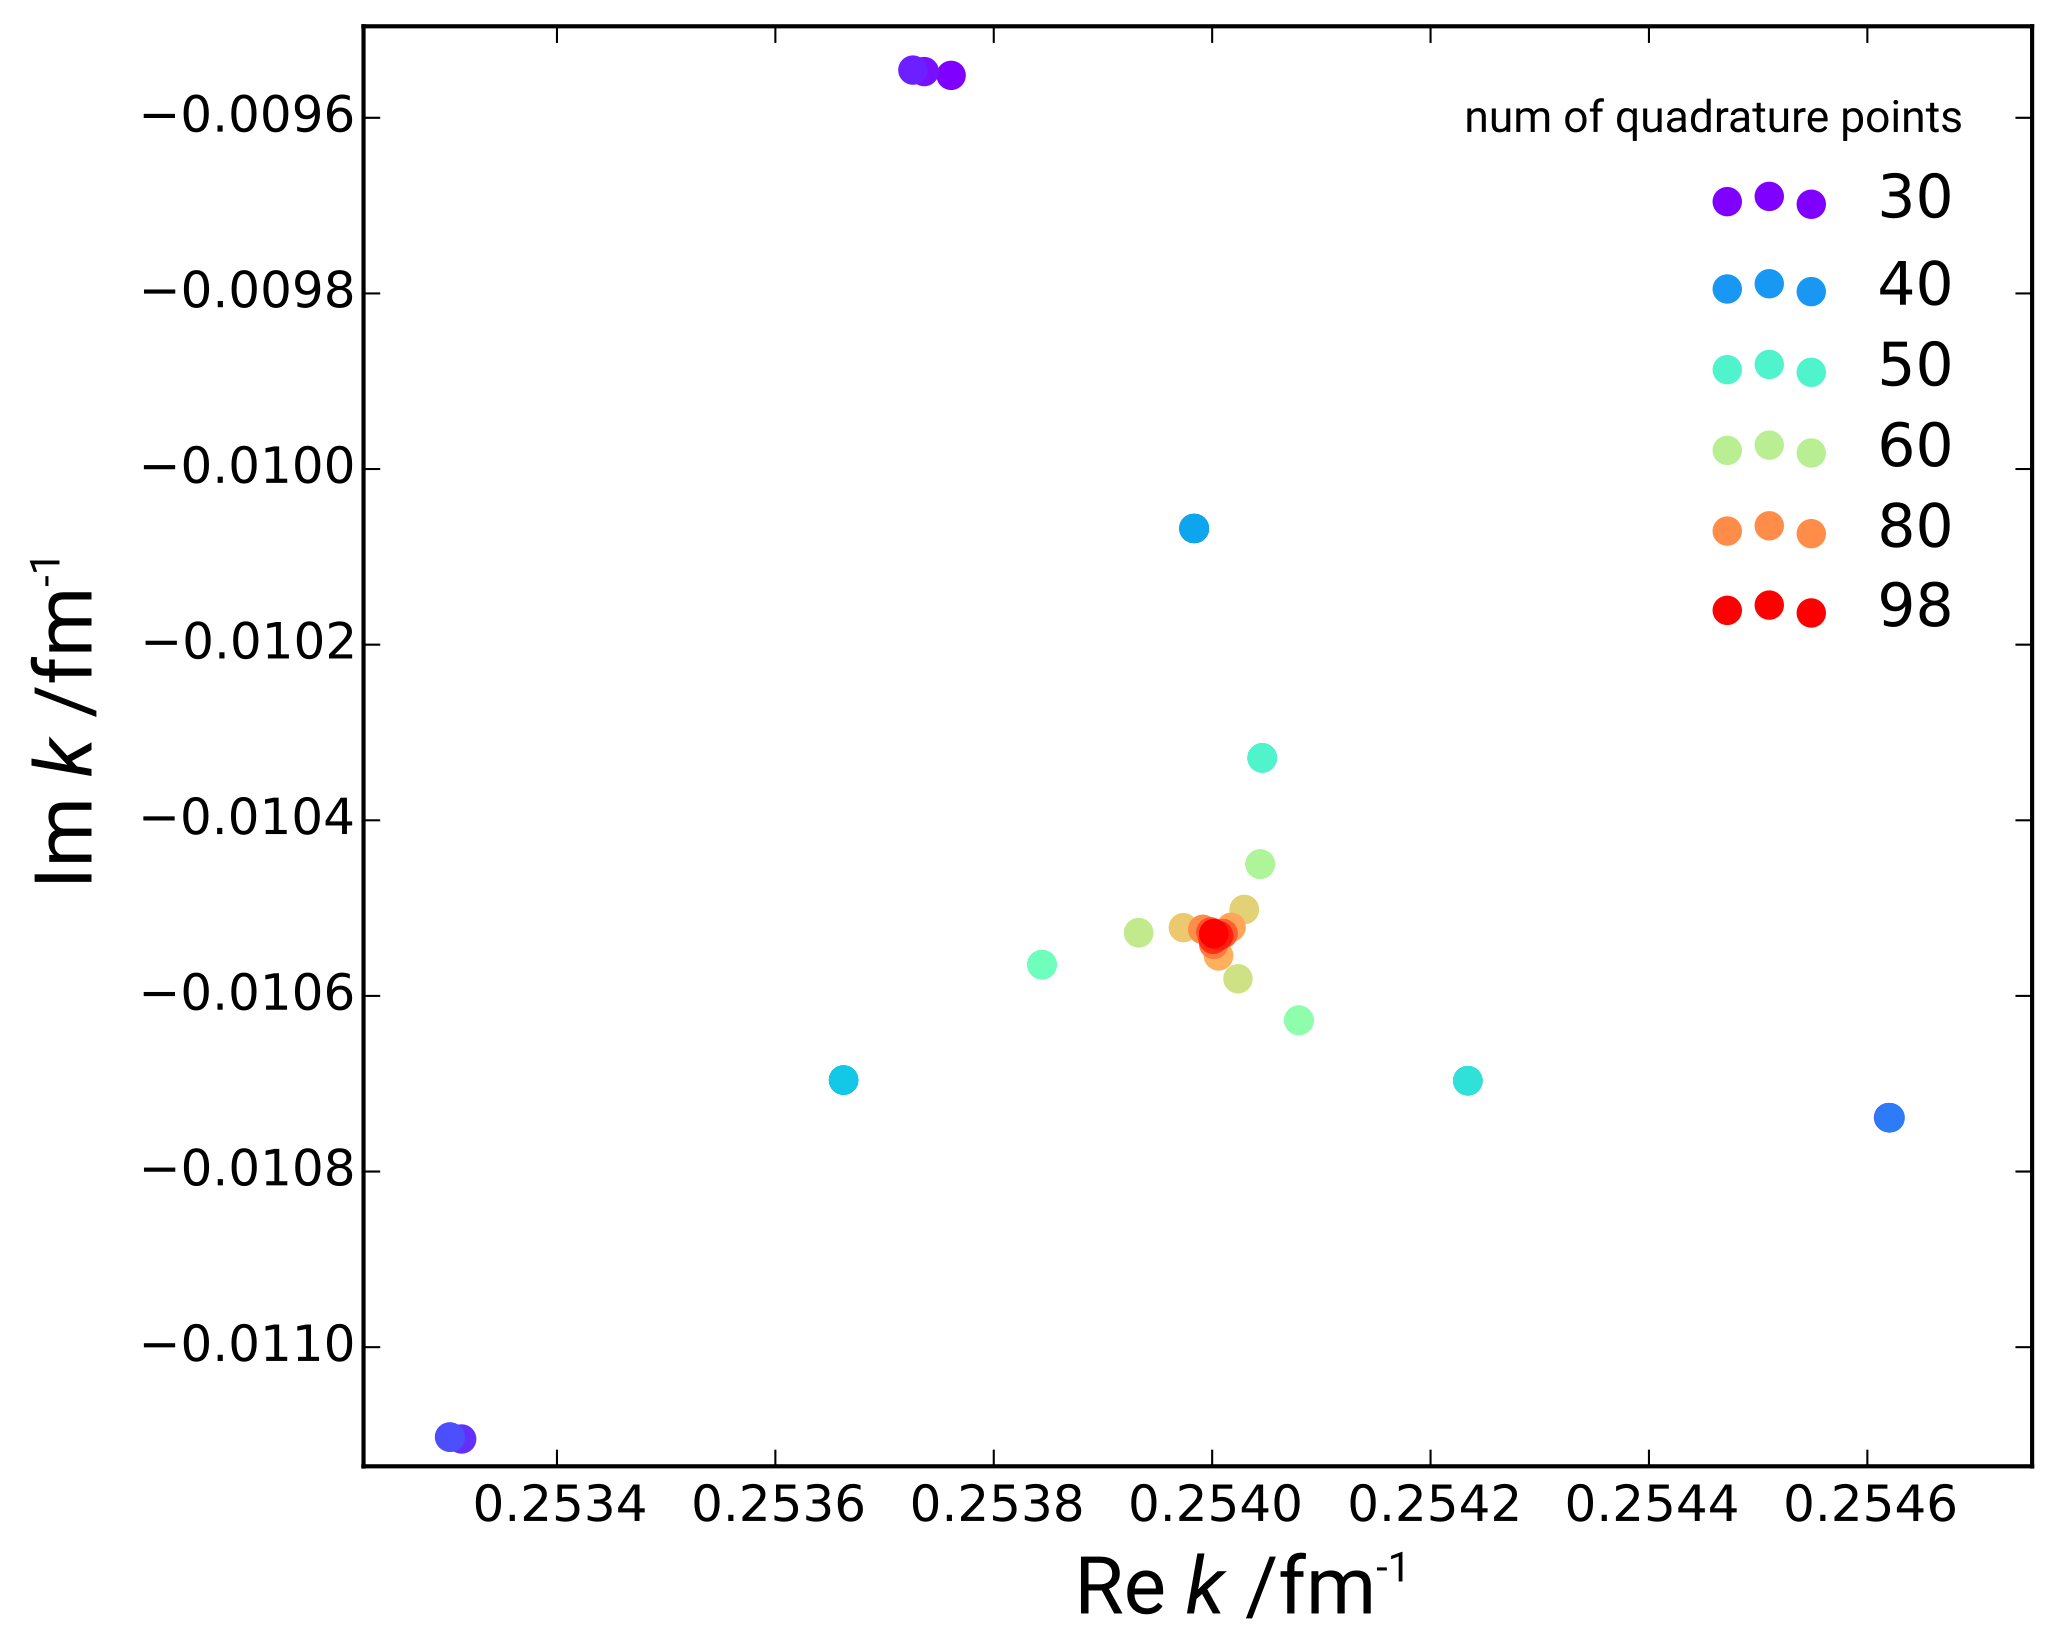
\includegraphics[width=.4\textwidth]{proj-convergence-count.pdf}
  \caption{Convergence of the resonant state with respect to the number of
    points in the discretized contour.  The legend has been trimmed down for
    clarity, but there are in fact many more colors in this plot than are
    shown in the legend.}
  \label{fig:convergence-count}
\end{figure}

To understand the uncertainty of our results, we must consider the various
potential sources of error.  It is possible that there may be insufficient
points in the discretization of the contour, leading to a poor result.  We
thus varied the number of discretization points and plotted the behavior of
the resonant momentum, shown in Figure \ref{fig:convergence-count}.  All other
parameters were kept constant for consistency.  The plot shows a clear trend
towards convergence, and by around 80 points the uncertainty is already well
within $10^{-4}\,\mathrm{fm}^{-1}$.  There is some peculiar behavior, however.
Firstly, there is a noticeable amount of clusterization of the points for
adjacent numbers of quadrature points, thus the convergence appears to occur
in large discrete steps.  Secondly, there is an emergent triangular pattern in
the plot, which indicates that there is some sort of approximate 3-fold
symmetry, perhaps an artifact of the contour's shape.  For future
investigations, it would be useful to use a completely different contour and
observe whether this pattern persists.

\begin{figure}
  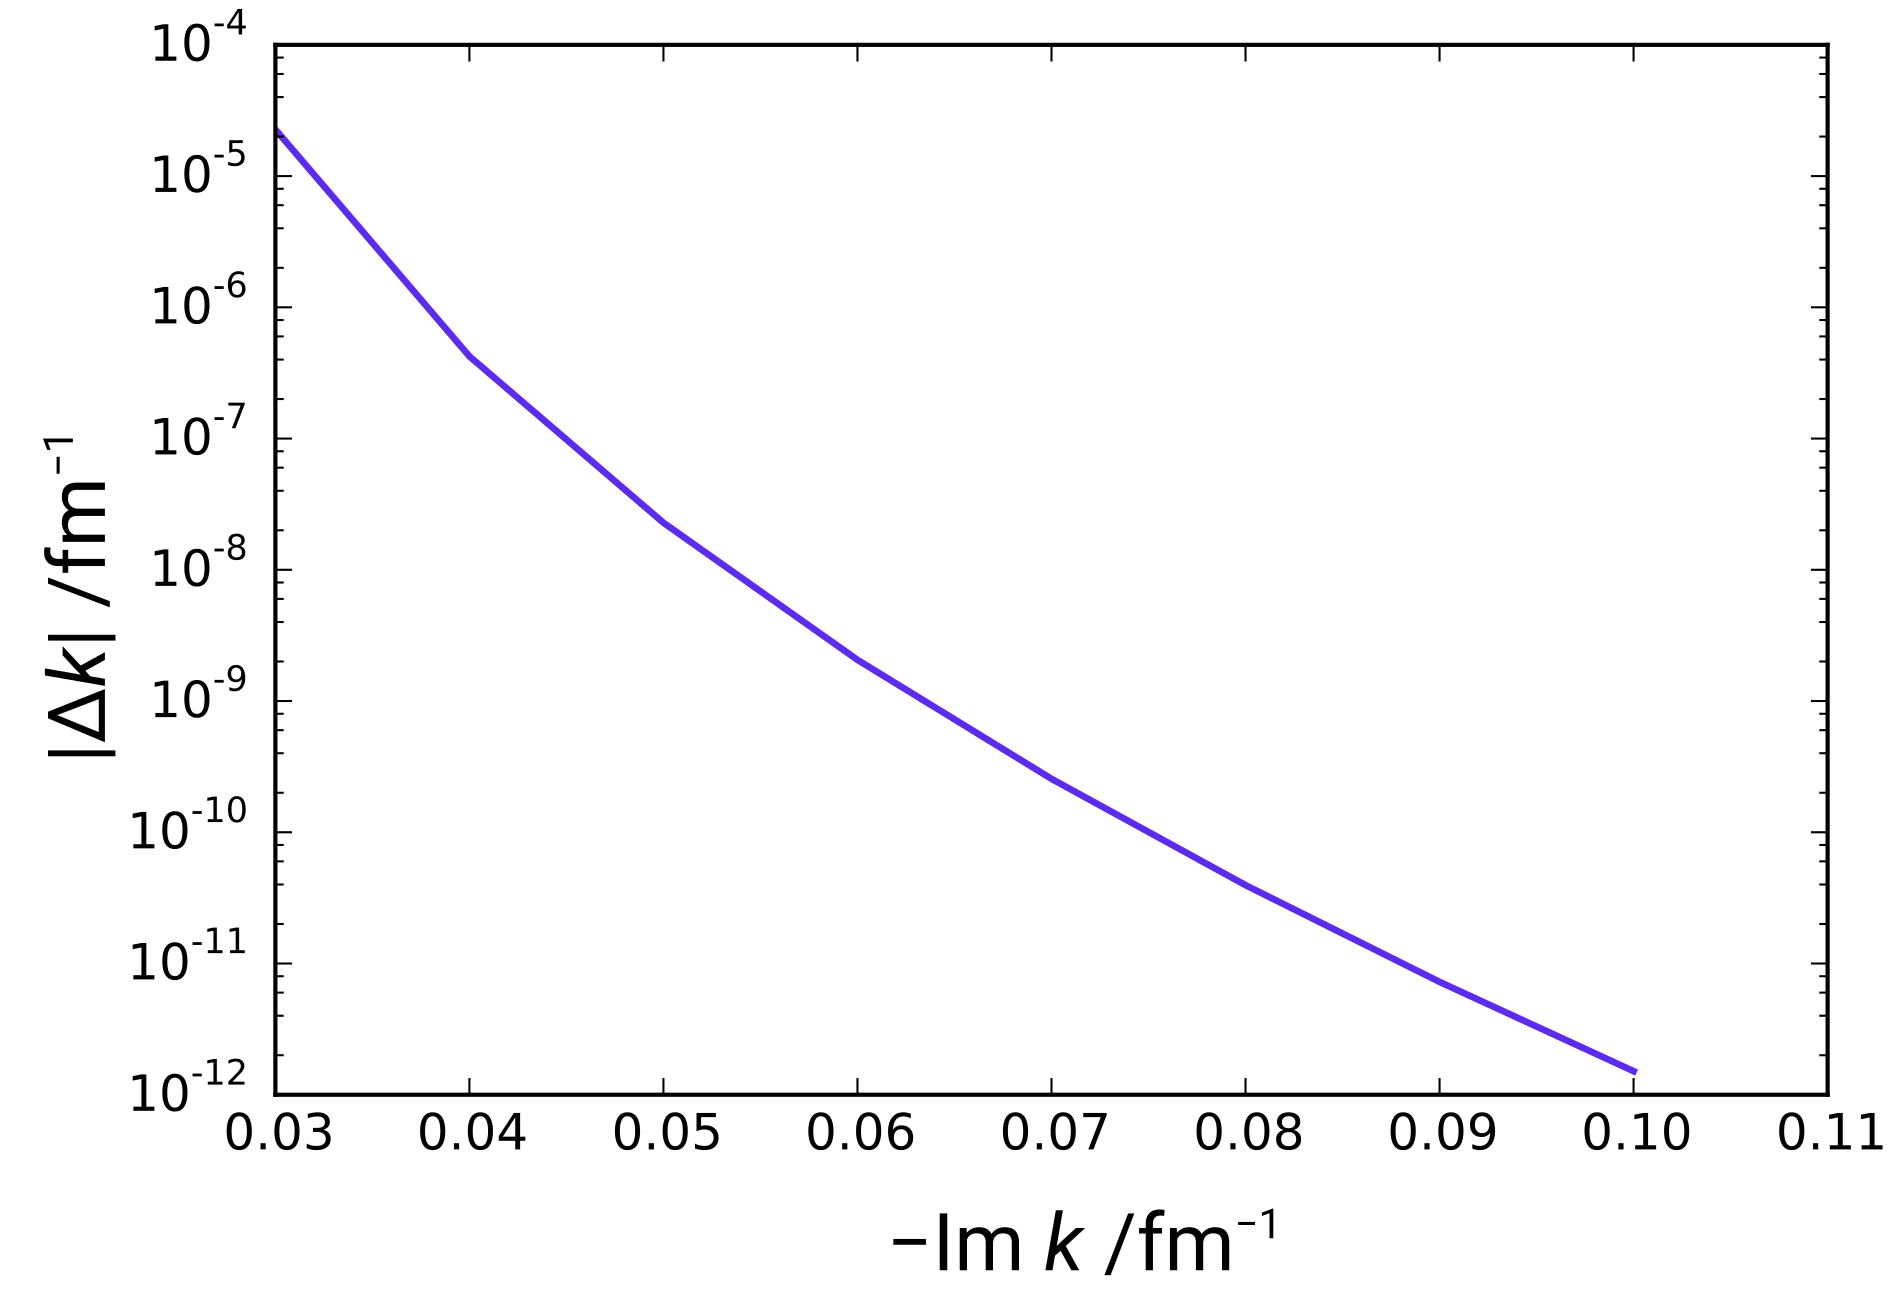
\includegraphics[width=.4\textwidth]{proj-convergence-height.pdf}
  \caption{Convergence of the resonant state with respect to the location of
    $k_{\text a}$.}
  \label{fig:convergence-height}
\end{figure}

Another potential source of error is in the shape of the contour.  Consider,
for example, the location of $k_{\text a}$.  To investigate this, we gradually
increased the imaginary component of $k_{\text a}$ from
$0.02\,\mathrm{fm}^{-1}$ to $0.10\,\mathrm{fm}^{-1}$ in steps of
$0.01\,\mathrm{fm}^{-1}$ and recorded how far the resonant momentum has shift
between each step of $k_{\text a}$.  This is plotted in Figure
\ref{fig:convergence-height}.  The result shows an exponential decrease in the
shift, suggesting that convergence is very rapid.  Eventually, the shift
reaches saturation once it becomes as small as the floating-point precision
(not shown in the figure).

The choice of $k_{\text{max}}$, similar to $k_{\text a}$, appears to make very
little difference beyond a certain point.  We found that
$k_{\text{max}} \ge 3\,\mathrm{fm}^{-1}$ appears to be more than sufficient.
We also found the results to be largely insensitive of $k_{\text b}$ -- the
resonant momentum fluctuations were below $10^{-9}\,\mathrm{fm}^{-1}$.

The radius cut-off, $R_{\text{max}}$ is also one of the adjustable parameters.
Similar to $k_{\text{max}}$, a minimum of $30\,\mathrm{fm}$ appeared to be
sufficient to ensure convergence.

\begin{figure}
  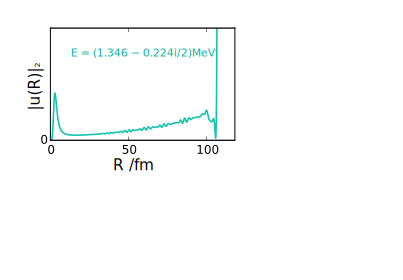
\includegraphics[width=.4\textwidth]{proj-l2-resonance-asymptotic.pdf}
  \caption{Poor asymptotics of the resonant state for the $\ell = 2$ partial
    wave, as indicated by the small oscillations as well as the sudden cliff
    at around $100\,\mathrm{fm}$.  The correct behavior is a steady
    exponential growth.}
  \label{fig:l2-resonance-asymptotic}
\end{figure}

We remark that despite the accurate momenta, the asymptotics of the
position-space wave functions are quite dubious: they can fluctuate
significantly depending on the parameters.  The method is able to compute the
position-space wave functions accurately for small radii, but as the radius
increases the accuracy decreases rapidly, as shown in Figure
\ref{fig:l2-resonance-asymptotic}.  This is alleviated somewhat by increasing
the number of discretization points, but it can quickly become very costly.
This is quite unlike the differential equation approach that we had previously
used where the asymptotics are nearly exact.  It may be possible to remedy
this by matching the boundary at some finite radius with the exact theoretical
result.

\subsection{Bound states}

\begin{figure}
  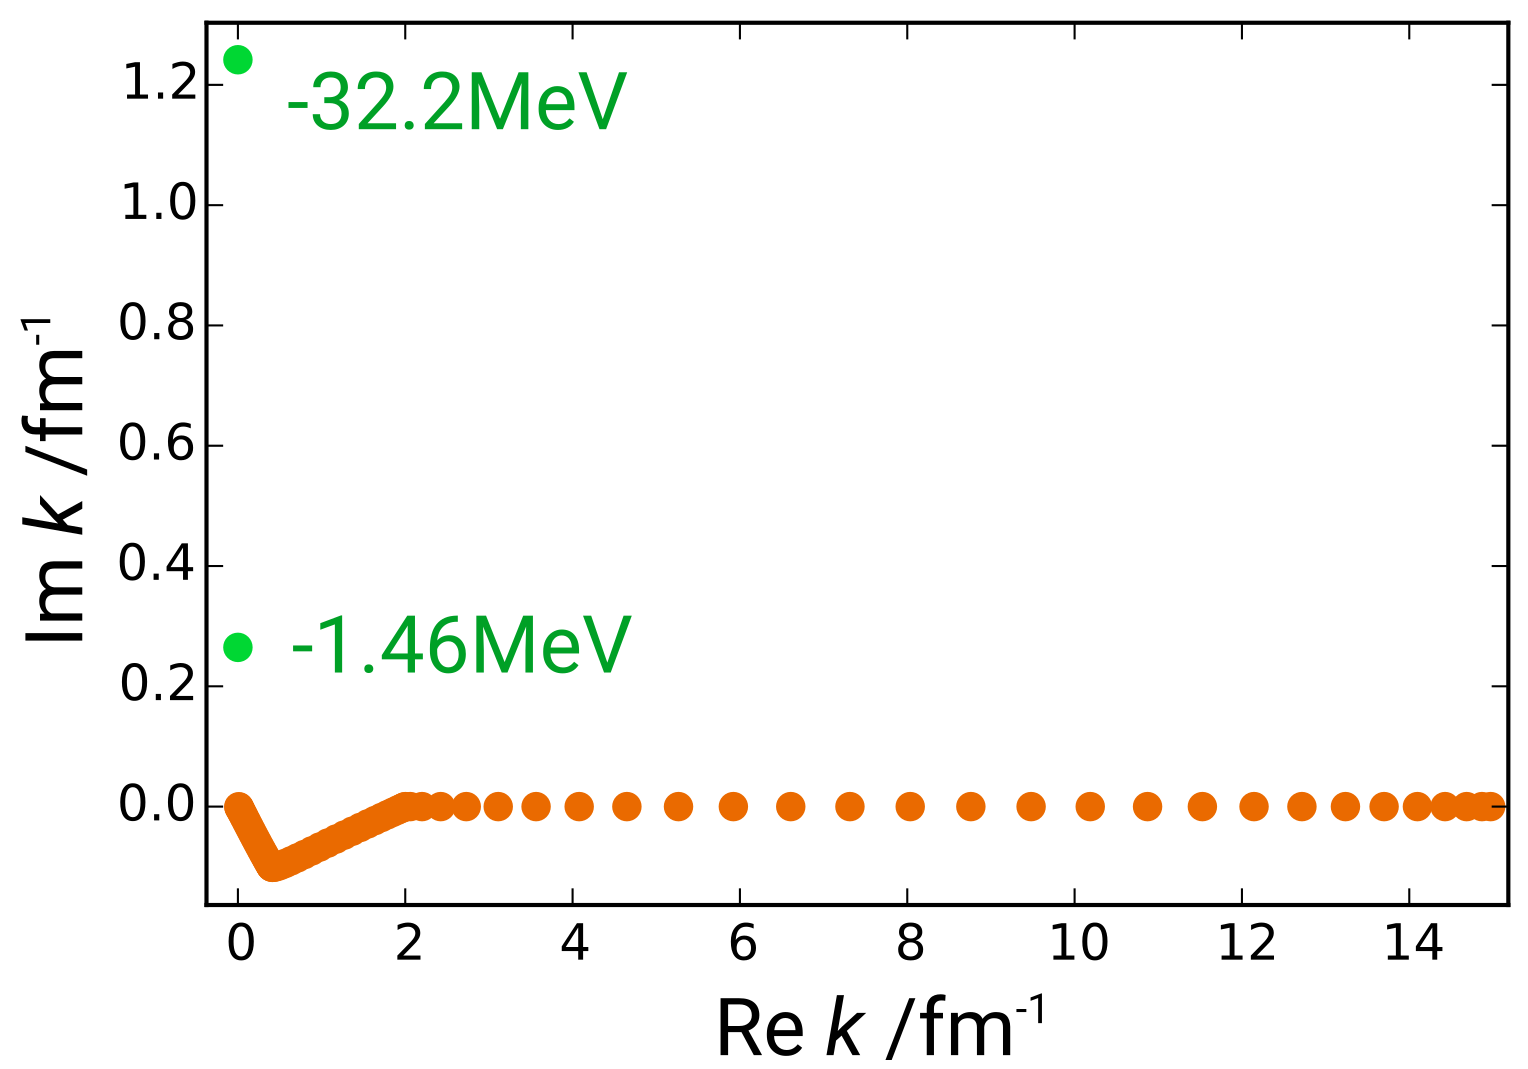
\includegraphics[width=.4\textwidth]{proj-l0.pdf}
  \caption{Momenta of the basis states for the $\ell = 0$ partial wave.}
  \label{fig:l0}
\end{figure}

\begin{figure}
  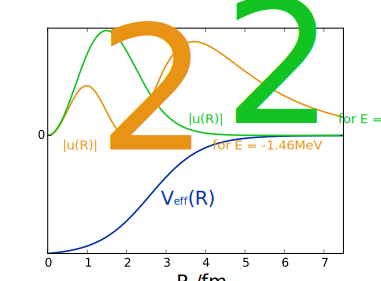
\includegraphics[width=.4\textwidth]{proj-l0-bound.pdf}
  \caption{Bound states for the $\ell = 0$ partial wave.}
  \label{fig:l0-bound}
\end{figure}

Interestingly, although not surprisingly, the same method works not only for
computing resonant states but also bound states.  We applied the same
technique as before to the $\ell = 0$ partial wave and were able to resolve
two bound states with energies $-32.2\,\mathrm{MeV}$ and $-1.46\,\mathrm{MeV}$
as shown in Figure \ref{fig:l0}.  The choice of the contour did not matter,
since bound states are always included in the basis, but we kept our original
contour for consistency.  The position-space wave functions of the bound
states are plotted in Figure \ref{fig:l0-bound}.

\section{Conclusions}

We have performed a calculation of the \textsuperscript{11}Be system using a
simple model and have extracted a resonant state with characteristics
consistent with our previous calculation through an entirely different
approach.  In doing so, we have demonstrated a technique for calculating
resonant states using a basis expansion approach, showing both its utility and
robustness.

For future investigations, there are several directions in which the project
can continue.  For one, it would be useful to further analyze the
uncertainities in the calculations due to other factors, such as the choice of
the quadrature method, the location of $k_0$, or the specified tolerance in
the calculation of $\tilde V$ matrix elements.

Another potential direction would be to incorporate more complicated
interactions, such surface Woods--Saxon potentials, or spin-orbit potentials.

It would be interesting to see how far the technique can be generalized.  One
could look into situations where the spherical symmetry is lost.  One could
also incorporate the long-ranged Coulomb potential into the Berggren basis.
There are some major complications that arise in this, for both theoretical
and numerical reasons.  For example, calculation of complex Coulomb wave
functions is not nearly as straightforward as calculating complex Bessel
functions.  The proof of the completeness relation for Coulombic potential is
also much more complicated than that of short-ranged
potentials.\cite{Michel2011}

\begin{acknowledgments}
  This work was developed as a project for the PHY982 Nuclear Dynamics course.
  We wish to thank the professors for their lectures and guidance throughout
  the course.  Although it was brief due to the half-semester schedule, the
  course was nonetheless helpful in broadening our knowledge in nuclear theory
  as well as gaining a firmer understanding of scattering theory.
\end{acknowledgments}
\bibliography{paper}
\end{document}
